\documentclass[a4paper,12pt]{article}
\usepackage[T1]{fontenc}
\usepackage[utf8]{inputenc}
\usepackage{lmodern}
\usepackage[french]{babel}
\usepackage{url,csquotes}
\usepackage[hidelinks,hyperfootnotes=false]{hyperref}
%\usepackage[titlepage]{polytechnique}
%\usepackage[titlepage,fancysections,pagenumber]{polytechnique}
\usepackage{float}
\usepackage{graphicx}
\usepackage{subfig}
\usepackage[margin=2cm]{geometry}

\usepackage{tcolorbox}
\usepackage{amsmath}
\usepackage{hyperref}

\usepackage{titlesec}

% Define the font size for subsection headings

%\setcounter{tocdepth}{}
%\usepackage[charter]{mathdesign}

%\setcounter{secnumdepth}{0}


\title{PHY361 DM1 \\
 Oscillations d’atomes piégés dans un potentiel parabolique}
%\subtitle{Stage linguistique à l'IFLS \\
%Formation Préparatoire}
\author{Isai GORDEEV et Imad BARAKAT\\
Promotion X2022, section Escrime}



\begin{document}

\maketitle



\section{Mesure par vol libre de la densité de probabilité de l’impulsion}
$$\hat H =  \hbar\omega(\hat a^{\dagger }\hat a + \frac12)$$
\subsection{}
Les états d'énergie propres d'opérateur $\hat H$
\begin{equation}\label{key}
	\hat H |\psi_n\rangle = E_n |\psi_n\rangle
\end{equation}
$$E_n = \hbar\omega(n+\frac 1 2) $$

\subsection{}

$a_0 = \displaystyle\sqrt{\frac{\hbar}{m\omega}} \sim 269 $ nm $ <\ \sim400$ nm, donc nous ne sommes pas capable. 

\subsection{}

L'image 1(a) est symétrique que correspond au formule de $\varphi_0$.\\

Dans l'image(a), $p_0 = 0$, après $T_v$ on voit bien que $\psi(p, t)$ s'est séparé.
C'est prévu par la théorie dans le cas libre. Calculons $ |\varphi_1(p)\rangle$ dans la représentation de l'impulsion $p$. 
Nous verrons aussi que l'image 2(a) correspond au formule de $\varphi_1 \sim p\exp(-p^2)$ \\ 







Après l'extinction du laser les atomes de Cs se sont comporté comme les particules libres. 
Enfin, pour calculer $T_v$ il faut mesurer l'impulsion moyenne de $|1\rangle$, ainsi regarder la coordonné de $p_1$. Comme il est demandé de calculer juste l'ordre de grandeur, on va prendre l'ordre de grandeur de $[p_1] = \sqrt 2\frac{\hbar}{a_0}$, $x = 200\mu m$

\begin{equation}
	T_v = \frac{mx}{[p_1]}  = \frac{mxa_0}{\sqrt 2\hbar} \sim 0.1 s
\end{equation}

\subsection{}
Prouvons que les opérateurs de $\hat x$ et $\hat p$ dans la représentation de l'impulsion $p$ sont 

\begin{equation}\label{key}
	\displaystyle\hat x \overset{P}{=} {\langle p|x|\psi \rangle} =  i\hbar\frac{\partial}{\partial p} 
\end{equation}

\begin{equation}\label{key}
		\displaystyle\hat p \overset{P}{=} {\langle p|x|\psi \rangle} = p
\end{equation}

L'opérateur de création appliquant à l'état fondamental. 
\begin{equation}
	|\psi_1\rangle = \hat a^\dagger|\psi_0\rangle  
\end{equation}

\begin{equation}
	|\psi_1\rangle = \left( \frac{a_0}{\hbar}\hat x - i\frac{1} {a_0}\hat p\right)|\psi_0\rangle 
\end{equation}

La représentation dans le X-espace. 
\begin{equation}
		\psi_1(x){=} \left( \frac{a_0}{\hbar}x -i\hbar \frac{1} {a_0}\frac{d}{dx} \right)\psi_0(x) 
\end{equation}


\begin{equation}
	{\displaystyle \psi (x)=\langle x|\psi \rangle =\int \!\!dp~\langle x|p\rangle \langle p|\psi \rangle =\int \!\!\frac{dp}{{\sqrt {2\pi \hbar }}}~{e^{ixp/\hbar }{{\varphi }}(p)},}
\end{equation}

\begin{equation}
	\begin{aligned}
	\displaystyle x\psi (x)&=\langle x|x|\psi \rangle =\int \!\!dp~\langle x|p\rangle \langle p|x|\psi \rangle =\int \!\!\frac{dp}{{\sqrt {2\pi \hbar }}}x{e^{ixp/\hbar }{{\varphi }}(p)} \overset{p.p.}{=} \\ 
	&\int \!\!\frac{dp}{{\sqrt {2\pi \hbar }}}{e^{ixp/\hbar }\underbrace{i\hbar\frac{d}{dp}\varphi(p)}_{\langle p|x|\psi \rangle}} 
\end{aligned}
\end{equation}

\begin{equation}
	\begin{aligned}
		\displaystyle -i\hbar\frac{d}{dx}\psi (x)&=\langle x|p|\psi \rangle =\int \!\!dp~\langle x|p\rangle \langle p|p|\psi \rangle =-i\hbar\frac{d}{dx}\int \!\!\frac{dp}{{\sqrt {2\pi \hbar }}}{e^{ixp/\hbar }{{\varphi }}(p)} {=} \\ 
		&\int \!\!\frac{dp}{{\sqrt {2\pi \hbar }}}{e^{ixp/\hbar }\underbrace{p\varphi(p)}_{\langle p|p|\psi \rangle}} 
	\end{aligned}
\end{equation}

Donc, nous avons dans le P-espace

\begin{equation}\label{eq}
		\varphi_1(p){=} \left( i\hbar\frac1{a_0}\frac{d}{dp} - i \frac{a_0} {\hbar}p \right)\varphi_0(p)
\end{equation}

\begin{equation}
	\varphi_1(p) = -\sqrt 2\left(\frac{a_0^2}{\pi \hbar^2}\right)^{\frac14}\left[i\frac{a_op}{\hbar}\exp\left(-\frac{a_0^2}{2\hbar^2}p^2\right)\right]
\end{equation}

\subsection{}


\begin{equation}\label{key}
	\varepsilon = -i\sqrt 2\left(\frac{a_0}{\hbar}\right)
\end{equation}

\subsection{}
Dessinons les deux graphiques schématiques $\varphi_0$, $\varphi_1$. Nous voyons que les données expérimentales correspondent à la théorie. 

\begin{figure}
	\centering
	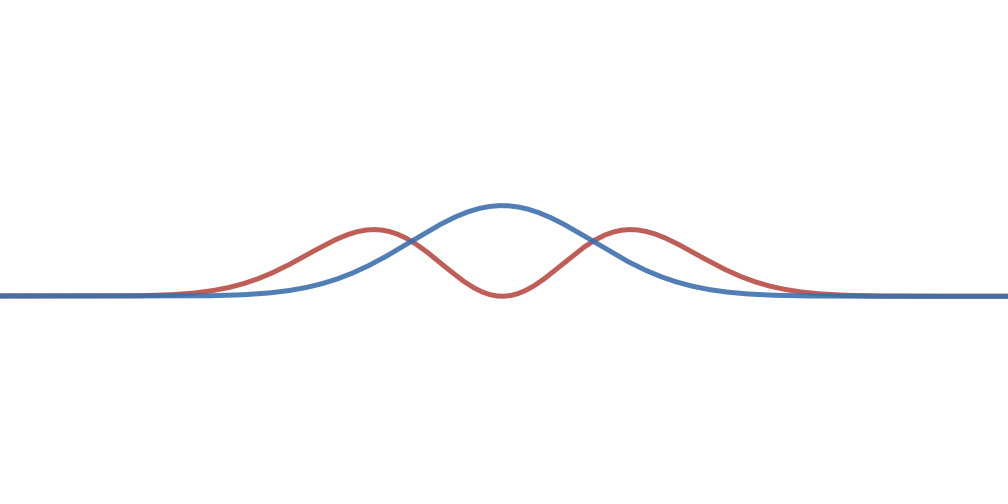
\includegraphics[width=0.5\textwidth]{1}
	\caption{blue – $\varphi_0$, rouge – $\varphi_1$ }
	\label{fig:image}
\end{figure}

\section{Préparation du système dans le premier état excité}
L'état fondamental c'est $\psi_0 = |0\rangle$. Le nouveau Hamiltonien $H_1$

\begin{equation}\label{key}
	H_1 = \frac{\hbar\Omega}{2}(|0\rangle\langle 1|+ |1\rangle\langle 0|)
\end{equation}

\subsection{}

Déterminons les états propres de $H_1$ 

\begin{equation}\label{key}
	\hat H_1|\psi_n\rangle = E_n|\psi_n\rangle
\end{equation}

\begin{equation}
	\frac{\hbar\Omega}{2}(|0\rangle\underbrace{\langle 1|\psi_n\rangle}_{\in C}+ |1\rangle\underbrace{\langle 0|\psi_n\rangle}_{\in C}) = E_n|\psi_n\rangle
\end{equation}

Nous remarquons que tout les états propres se constituent seulement de deux états de $\hat H_0$, $|0\rangle$,$ |1\rangle$, donc 

\begin{equation}\label{key}
	|\psi_n\rangle = a_0 |0\rangle + a_1 |1\rangle
\end{equation}

La normalisation de $\langle\psi_n|\psi_n\rangle$ nous donne 

\begin{equation}\label{key}
	a_0^2 + a_1^2 = 1
\end{equation}

La définition de $\langle 0|\psi_n\rangle = a_1$ et  $\langle 1|\psi_n\rangle = a_0$ nous donne 

\begin{equation}\label{key}
	a_0^2 = a_1^2
\end{equation}

Nous avons deux paires de solutions

\begin{equation}\label{key}
	(a_0, a_1) = (\frac{1}{\sqrt2}, \frac{1}{\sqrt2})
\end{equation}
\begin{equation}\label{key}
	(a_0, a_1) = (\frac{1}{\sqrt2}, -\frac{1}{\sqrt2})
\end{equation}

Donc, les états propres 

\begin{equation}\label{key}
	|\tilde \psi_0\rangle = \frac{|0\rangle + |1\rangle}{\sqrt2}\ \ \ E_0 = \frac{\hbar\Omega}{2}
\end{equation}

\begin{equation}\label{key}
	|\tilde \psi_1\rangle = \frac{|0\rangle - |1\rangle}{\sqrt2}\ \ \ \ E_1 =- \frac{\hbar\Omega}{2}
\end{equation}

\subsection{}

\begin{equation}\label{key}
	|0\rangle = \frac{|\tilde \psi_1\rangle + |\tilde \psi_0\rangle}{\sqrt2}
\end{equation}

\begin{equation}\label{key}
	|1\rangle = \frac{|\tilde \psi_0\rangle - |\tilde \psi_1\rangle}{\sqrt2}
\end{equation}

Évolution de $|0\rangle$ est donnée par l'équation de Sh.

\begin{equation}\label{key}
	i\hbar\frac{\partial}{\partial t}|\tilde \psi_n(t)\rangle = \hat H_1|\tilde \psi_n(t)\rangle
\end{equation}

\begin{equation}\label{key}
	|\tilde \psi_n(t)\rangle = |\tilde \psi_n(0)\rangle \exp\left(-\frac{iE_nt}{\hbar}\right)
\end{equation}

\begin{equation}\label{key}
	|\psi_0(t)\rangle = \frac{|\tilde \psi_0(0)\rangle \exp\left(-{\frac i 2\Omega t}\right) + |\tilde \psi_1(0)\rangle \exp\left({\frac i 2\Omega t}\right)}{\sqrt 2}
\end{equation}



\subsection{}

\begin{equation}\label{key}
	|\psi_0(t)\rangle = \cos\left(\frac 12\Omega t\right)|0\rangle -i \sin\left(\frac 12\Omega t\right)|1\rangle
\end{equation}

\subsection{}

Une mesure de $|1\rangle$ est faite avec une probabilité 
\begin{equation}\label{key}
	P(t) = \sin^2\left(\frac 12\Omega t\right) = \frac 12 -\frac{\cos (\Omega t)}{2}
\end{equation}

Donc, $T = \displaystyle\frac{2\pi}{\Omega}$

\subsection{}

Il faut éteindre le laser dans le moment quand $P(t) = 1$ 

\begin{equation}\label{key}
	\cos (\Omega t) = -1
\end{equation}

\begin{equation}\label{key}
	t = \frac{T}2(1+2n)
\end{equation}


\section{Préparation d’un état non stationnaire}

Dans cette partie, on choisit d’interrompre l’application du second faisceau laser discuté à la partie précédente à l’instant $T/4$.

\subsection{}

\begin{equation}\label{key}
	|\psi_0(t)\rangle = \cos\left(\frac 18\Omega T\right)|0\rangle -i \sin\left(\frac 18\Omega T\right)|1\rangle
\end{equation}

\begin{equation}\label{key}
	|\psi_0(t)\rangle = \frac{1}{\sqrt 2}(|0\rangle - i|1\rangle)
\end{equation}

\subsection{}

Après le moment T, nous avons le changement d'opérateur $\hat H$, par conséquent 
\begin{equation}\label{key}
	|\psi_0(\frac T 4 + t)\rangle = \frac{1}{\sqrt 2}(\exp(-i\frac{wt}{2})|0\rangle - i\exp(-i\frac{3wt}{2})|1\rangle)
\end{equation}


\subsection{}
Il y a deux cas 

\subsubsection{}
$t < \frac T 4$



\begin{equation}
	\langle p|\psi_0(t)\rangle = \varphi(p, t) = \cos\left(\frac 12\Omega t\right)\varphi_0-i \sin\left(\frac 12\Omega t\right)\varphi_1
\end{equation}

\begin{equation}
	 \varphi(p, t) = \cos\left(\frac 12\Omega t\right)\varphi_0-i \sin\left(\frac 12\Omega t\right)\epsilon p \varphi_0
\end{equation}

\begin{equation}
	\varphi^2(p, t) =\left[\cos^2\left(\frac 12\Omega t\right)+\sin^2\left(\frac 12\Omega t\right)\epsilon^2 p^2 \right]\varphi^2_0(p)
\end{equation}

\subsubsection{}
$t > \frac T 4$

\begin{equation}
	\langle p|\psi_0(t)\rangle = \varphi(p, t) = \frac{1}{\sqrt 2}(\exp(-i\frac{wt}{2})\varphi_0(p) - i\exp(-i\frac{3wt}{2})\varphi_1(p))
\end{equation}

\begin{equation}
	\varphi(p, t) = \frac{1}{\sqrt 2}(\exp(-i\frac{wt}{2})\varphi_0(p) - i\exp(-i\frac{3wt}{2})\epsilon p\varphi_0(p))
\end{equation}


\begin{equation}
	\varphi^2(p, t) =\frac{1}{2}\left(1+(\epsilon p)^2 - 2\epsilon p \sin\left(\frac {wt} 2\right)\right) \varphi^2_0(p)
\end{equation}

\subsection{}

Nous voyons que dans le graphique c'est une fonction périodique qui fait des oscillation autour d'un point fixe, que correspond à la fonction obtenue dans (41). 

En moment de $\tau = 8\tau_0$ la courbe se met dans la position initiale, donc 

\begin{equation}\label{key}
	4w\tau_0 = 2\pi \rightarrow \tau_0 = \frac {1} {4\nu} = 2.7\mu s
\end{equation}



\end{document}